\documentclass{article}
\usepackage{tikz}
%\pagecolor{darkgray}
\pagecolor{right color=red!80,left color=blue!20}
\usetikzlibrary{3d}
\begin{document}
%\color{blue!20!black!30!green}

%\title{Un paseo aleatorio: \textit{La edición de código como práctica artística.} {}}
%\title{Un paseo aleatorio: \textit{Live Coding} con \LaTeX{}}
%\title{La edición de código en vivo como práctica artística.{}}\\

%\title{Sombreado:\textit{Código creativo} con \LaTeX{}}
%\author{x_x}

\maketitle

%\colorbox{green}{\color{white}live coding with \Latex{}}
%\colorbox{green}{\color{red}.}
%\colorbox{green}{\color{red}.}
%\colorbox{green}\color{red}
\begin{center}
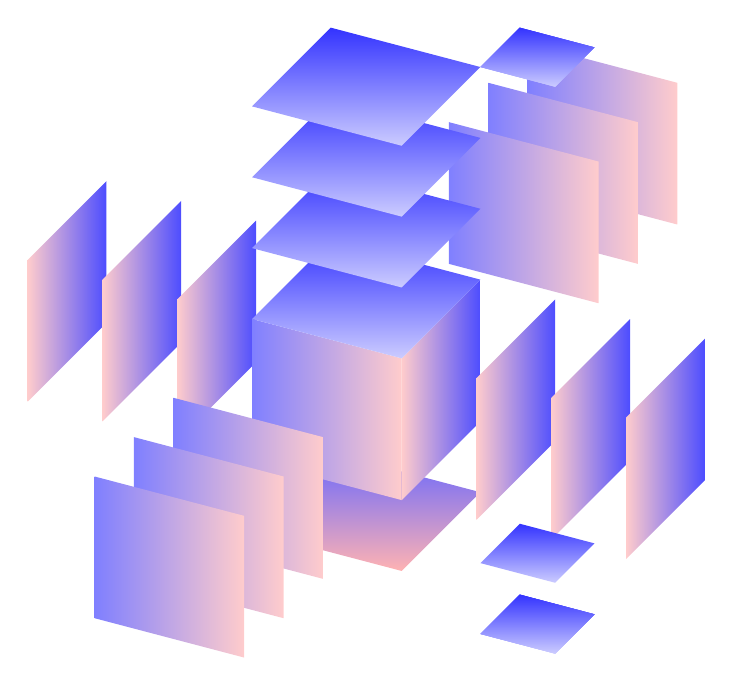
\begin{tikzpicture}[x  = {(0.5cm,0.5cm)},
                    y  = {(0.95cm,-0.25cm)},
                    z  = {(0cm,0.9cm)}]
\begin{scope}[canvas is yx plane at z=-2]
\shade[top color=blue!60,bottom color=red!30] (-1,-1) rectangle (1,1);
\end{scope}

\begin{scope}[canvas is xz plane at y=-4]
  \shade[right color=blue!70,left color=red!20] (-1,-1) rectangle (1,1);
\end{scope}
\begin{scope}[canvas is xz plane at y=-3]
  \shade[right color=blue!70,left color=red!20] (-1,-1) rectangle (1,1);
\end{scope}
\begin{scope}[canvas is xz plane at y=-2]
  \shade[right color=blue!70,left color=red!20] (-1,-1) rectangle (1,1);
\end{scope}

\begin{scope}[canvas is xz plane at y=1]
  \shade[right color=blue!70,left color=red!20] (-1,-1) rectangle (1,1);
\end{scope}
\begin{scope}[canvas is xz plane at y=2]
  \shade[right color=blue!70,left color=red!20] (-1,-1) rectangle (1,1);
\end{scope}




\begin{scope}[canvas is xz plane at y=3]
  \shade[right color=blue!70,left color=red!20] (-1,-1) rectangle (1,1);
\end{scope}



\begin{scope}[canvas is yz plane at x=6]
  \shade[left color=blue!50,right color=red!20] (-1,-1) rectangle (1,1);
\end{scope}
\begin{scope}[canvas is yz plane at x=5]
  \shade[left color=blue!50,right color=red!20] (-1,-1) rectangle (1,1);
\end{scope}
\begin{scope}[canvas is yz plane at x=4]
  \shade[left color=blue!50,right color=red!20] (-1,-1) rectangle (1,1);
\end{scope}



\begin{scope}[canvas is yz plane at x=-1]
  \shade[left color=blue!50,right color=red!20] (-1,-1) rectangle (1,1);
\end{scope}
\begin{scope}[canvas is yz plane at x=-3]
  \shade[left color=blue!50,right color=red!20] (-1,-1) rectangle (1,1);
\end{scope}
\begin{scope}[canvas is yz plane at x=-4]
  \shade[left color=blue!50,right color=red!20] (-1,-1) rectangle (1,1);
\end{scope}

\begin{scope}[canvas is xz plane at y=4]
  \shade[right color=blue!70,left color=red!20] (-1,-1) rectangle (1,1);
\end{scope}

% yx



\begin{scope}[canvas is yx plane at z=1]
  \shade[top color=blue!80,bottom color=blue!20] (-1,-1) rectangle (1,1);
\end{scope}
\begin{scope}[canvas is yx plane at z=2]
  \shade[top color=blue!80,bottom color=blue!20] (-1,-1) rectangle (1,1);
\end{scope}
\begin{scope}[canvas is yx plane at z=3]
  \shade[top color=blue!80,bottom color=blue!20] (-1,-1) rectangle (1,1);
\end{scope}
\begin{scope}[canvas is yx plane at z=4]
  \shade[top color=blue!80,bottom color=blue!20] (-1,-1) rectangle (1,1);
\end{scope}


\begin{scope}[canvas is yx plane at z=4]
  \shade[top color=blue!80,bottom color=blue!20] (2,2) rectangle (1,1);
\end{scope}
\begin{scope}[canvas is yx plane at z=4]
  \shade[top color=blue!80,bottom color=blue!20] (2,2) rectangle (1,1);
\end{scope}
\begin{scope}[canvas is yx plane at z=4]
  \shade[top color=blue!80,bottom color=blue!20] (2,2) rectangle (1,1);
\end{scope}

\begin{scope}[canvas is yx plane at z=-4]
  \shade[top color=blue!80,bottom color=blue!20] (2,2) rectangle (1,1);
\end{scope}
\begin{scope}[canvas is yx plane at z=-4]
  \shade[top color=blue!80,bottom color=blue!20] (2,2) rectangle (1,1);
\end{scope}
\begin{scope}[canvas is yx plane at z=-4]
  \shade[top color=blue!80,bottom color=blue!20] (2,2) rectangle (1,1);
\end{scope}

\begin{scope}[canvas is yx plane at z=-3]
  \shade[top color=blue!80,bottom color=blue!20] (2,2) rectangle (1,1);
\end{scope}
\begin{scope}[canvas is yx plane at z=-4]
  \shade[top color=blue!80,bottom color=blue!20] (2,2) rectangle (1,1);
\end{scope}


\begin{scope}[canvas is yz plane at x=-5]
  \shade[left color=blue!50,right color=red!20] (-1,-1) rectangle (1,1);
\end{scope}




\end{tikzpicture}
\end{center}
%\colorbox{green}{\color{white}live coding with \Latex{}}
\begin{center}
%\title{confinamiento 2020.{}}\\
%\title{(Posible cover de cover posible XD){}}

%\author{x_x}
\end{center}
%\colorbox{red}

\maketitle
\end{document}
